\documentclass[aspectratio=169,10pt]{beamer}

\usetheme{Madrid}
\usecolortheme{seahorse}
\setbeamertemplate{navigation symbols}{}
\setbeamertemplate{footline}[frame number]

\usepackage{amsmath,amssymb,booktabs,array}
\usepackage{tikz}
\usetikzlibrary{arrows.meta,positioning,shapes.geometric,fit,calc}
\usepackage{listings}
\usepackage{xcolor}
\usepackage{hyperref}

\definecolor{codebg}{RGB}{248,248,248}
\definecolor{darkblue}{RGB}{0,65,120}
\definecolor{darkgreen}{RGB}{0,105,70}
\definecolor{warnorange}{RGB}{190,110,0}

\hypersetup{colorlinks=true,linkcolor=darkblue,urlcolor=darkblue}

\lstdefinestyle{pythonstyle}{
    language=Python,
    basicstyle=\ttfamily\scriptsize,
    keywordstyle=\color{darkblue}\bfseries,
    commentstyle=\color{darkgreen},
    stringstyle=\color{warnorange},
    showstringspaces=false,
    columns=fullflexible,
    backgroundcolor=\color{codebg},
    frame=single,
    rulecolor=\color{black!15},
    breaklines=true
}
\lstset{style=pythonstyle}

\newcommand{\code}[1]{\texttt{#1}}
\newcommand{\checkitem}{\textcolor{darkgreen}{\Large$\checkmark$}\;}
\newcommand{\warnitem}{\textcolor{warnorange}{\Large$\triangle$}\;}

\title[L01: PF Fundamentals]{L01 -- Power Flow Fundamentals}
\subtitle{Foundations Lecture Series}
\author{Course Instructor}
\institute{Microgrid 3-phase Security AI Project}
\date{Foundations Lecture 1}

\begin{document}

% ============================================================
\begin{frame}
  \titlepage
  \vspace{-0.8em}
  \begin{center}
    \small Keywords: bus, branch, per-unit, Y-bus, Newton-Raphson, slack/PV/PQ
  \end{center}
\end{frame}

% ============================================================
\begin{frame}{Lecture roadmap}
\begin{enumerate}
  \item Why power flow? What problem are we actually solving?
  \item The setup: buses, branches, per-unit, bus types
  \item The math: Y-bus and the power-flow equations
  \item Solving it: Newton-Raphson in one slide
  \item A worked three-bus example
  \item pandapower preview: how this looks in code
  \item Limits and what comes in L02--L04
\end{enumerate}
\vspace{0.6em}
\begin{block}{What you will leave with}
The ability to write down the power-flow equations from a one-line diagram, classify each bus correctly, and run \code{pp.runpp(net)} understanding what every line of input and output means.
\end{block}
\end{frame}

% ============================================================
\section*{1. Why power flow?}

\begin{frame}{The grid as a giant electrical circuit}
\begin{columns}[T]
\column{0.55\textwidth}
\begin{itemize}
  \item Sources (generators, PV, batteries) and sinks (loads) connected by transmission and distribution lines.
  \item Continuous instantaneous balance: $\sum P_{\text{gen}} = \sum P_{\text{load}} + P_{\text{losses}}$.
  \item Operators care about voltages, currents, and limits in \emph{steady state}.
  \item \emph{Power flow} = solve for the steady-state operating point given the loads and generator setpoints.
\end{itemize}
\column{0.42\textwidth}
\begin{block}{What it is not}
Not dynamics (no rotor angle ODEs). Not protection (no fault current calculation). Not market clearing (no economic dispatch). \emph{Just the snapshot.}
\end{block}
\end{columns}
\end{frame}

% ============================================================
\begin{frame}{What operators actually need to know}
\begin{itemize}
  \item Voltage at every bus -- magnitude and angle.
  \item Active and reactive power flow on every line and transformer.
  \item Are all voltages between $0.95$ and $1.05$ pu?
  \item Is any line loaded above $100\%$ of its current rating?
  \item How much P and Q is the swing generator actually picking up?
\end{itemize}
\vspace{0.5em}
\begin{block}{Use cases}
\begin{itemize}
  \item Dispatch / operations planning
  \item Contingency analysis (this course)
  \item Network expansion planning
  \item Market clearing (security-constrained OPF)
  \item Hosting capacity studies for DER
\end{itemize}
\end{block}
\end{frame}

% ============================================================
\begin{frame}{Power flow in one slide}
\begin{block}{Given}
\begin{itemize}
  \item Network topology (which bus connects to which through what)
  \item Line / transformer impedances
  \item Generator and load setpoints
\end{itemize}
\end{block}
\begin{block}{Find}
\begin{itemize}
  \item Voltage magnitude $|V_i|$ and angle $\theta_i$ at every bus
\end{itemize}
\end{block}
\begin{block}{Then derive}
\begin{itemize}
  \item Currents and active/reactive power on every branch
  \item Total losses
  \item Generator outputs at the slack bus
\end{itemize}
\end{block}
\end{frame}

% ============================================================
\section*{2. The setup}

\begin{frame}{Buses, branches, generators, loads}
\centering
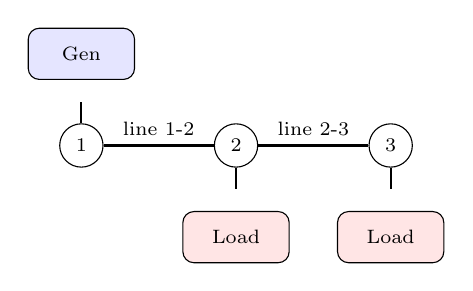
\begin{tikzpicture}[node distance=1.0cm and 1.4cm, every node/.style={font=\scriptsize}]
\tikzset{bus/.style={draw, circle, minimum size=0.55cm, fill=white}}
\tikzset{dev/.style={draw, rounded corners, align=center, minimum width=1.35cm, minimum height=0.65cm}}
\node[bus] (b1) {1};
\node[bus, right=of b1] (b2) {2};
\node[bus, right=of b2] (b3) {3};
\node[dev, above=0.55cm of b1, fill=blue!10] {Gen};
\node[dev, below=0.55cm of b2, fill=red!10] {Load};
\node[dev, below=0.55cm of b3, fill=red!10] {Load};
\draw[thick] (b1) -- node[above]{line 1-2} (b2);
\draw[thick] (b2) -- node[above]{line 2-3} (b3);
\draw[thick] (b1) -- ++(0,0.55);
\draw[thick] (b2) -- ++(0,-0.55);
\draw[thick] (b3) -- ++(0,-0.55);
\end{tikzpicture}
\vspace{0.6em}
\begin{itemize}
  \item \textbf{Bus} -- a node. Where things connect.
  \item \textbf{Branch} -- a line, transformer, or switch connecting two buses.
  \item \textbf{Generator} -- power source. Injects $P_g, Q_g$ into a bus.
  \item \textbf{Load} -- power sink. Draws $P_d, Q_d$ from a bus.
  \item \textbf{State variables} at each bus: $|V_i|, \theta_i$.
\end{itemize}
\end{frame}

% ============================================================
\begin{frame}{Per-unit system: why and how}
\textbf{Why}
\begin{itemize}
  \item A transformer changes voltage levels. Without per-unit, every quantity has different units on each side. Confusing.
  \item In per-unit, the same line impedance has the same value on both sides of a transformer.
  \item Per-unit voltage is approximately $1.0$ everywhere when the system is healthy.
\end{itemize}
\vspace{0.4em}
\textbf{How}
\begin{itemize}
  \item Pick $S_{\text{base}}$ (e.g., 100 MVA) and $V_{\text{base}}$ per voltage zone.
  \item Compute $Z_{\text{base}} = V_{\text{base}}^2 / S_{\text{base}}$, $I_{\text{base}} = S_{\text{base}}/(\sqrt{3}\, V_{\text{base}})$.
  \item Divide every quantity by its base: $V_{pu} = V/V_{\text{base}}$, etc.
\end{itemize}
\begin{alertblock}{Rule of thumb}
If you see ``$V_i = 0.96$ pu'', that means $96\%$ of nominal voltage --- usually borderline-low.
\end{alertblock}
\end{frame}

% ============================================================
\begin{frame}{Bus types: slack, PV, PQ}
\centering
\small
\begin{tabular}{lllll}
\toprule
Type & Known & Unknown & Physical interpretation & Number per system \\
\midrule
\textbf{Slack} & $|V|, \theta$ & $P, Q$ & Reference + absorbs imbalance & exactly 1 \\
\textbf{PV} & $P, |V|$ & $\theta, Q$ & Generator with voltage control & several \\
\textbf{PQ} & $P, Q$ & $|V|, \theta$ & Load or fixed-output source & many \\
\bottomrule
\end{tabular}
\vspace{0.8em}
\begin{block}{Why this taxonomy}
Each bus contributes two unknowns ($|V_i|, \theta_i$) and two equations ($P_i, Q_i$).
\begin{itemize}
  \item At a PQ bus we know $P$ and $Q$ from the load, so we solve for $|V|$ and $\theta$.
  \item At a PV bus the generator controls $|V|$; $Q$ is whatever the generator must supply.
  \item The slack bus fixes $\theta$ as the angle reference and picks up losses.
\end{itemize}
\end{block}
\end{frame}

% ============================================================
\section*{3. The math}

\begin{frame}{Bus admittance matrix $Y_{\text{bus}}$}
For each line between bus $i$ and bus $j$ with series admittance $y_{ij} = 1/(R + jX)$:
\begin{align*}
Y_{ii} &= \sum_{j \neq i} y_{ij} + y_{i,\text{shunt}} \\
Y_{ij} &= -y_{ij}, \quad j \neq i
\end{align*}
\vspace{0.4em}
Stack into a complex $N \times N$ matrix:
\begin{equation*}
Y_{\text{bus}} = G + jB \quad \in \mathbb{C}^{N \times N}
\end{equation*}
\begin{block}{Properties}
\begin{itemize}
  \item Symmetric: $Y_{ij} = Y_{ji}$.
  \item Sparse for real networks (each bus connects to a few neighbours).
  \item Pre-computed once at the start of a power-flow solve.
\end{itemize}
\end{block}
\end{frame}

% ============================================================
\begin{frame}{The power-flow equations}
The current injected at bus $i$ is $I_i = \sum_j Y_{ij} V_j$. The complex power injection is
\begin{equation*}
S_i = P_i + jQ_i = V_i \, I_i^{\,*} = V_i \sum_j Y_{ij}^{\,*} \, V_j^{\,*}.
\end{equation*}
Writing $V_i = |V_i| \angle \theta_i$ and $Y_{ij} = |Y_{ij}|\angle \alpha_{ij}$ and expanding:
\begin{align*}
P_i &= \sum_j |V_i| |V_j| |Y_{ij}| \cos(\theta_i - \theta_j - \alpha_{ij}) \\
Q_i &= \sum_j |V_i| |V_j| |Y_{ij}| \sin(\theta_i - \theta_j - \alpha_{ij})
\end{align*}
\begin{alertblock}{The key observation}
These equations are \emph{nonlinear} in $|V|$ and $\theta$ --- products of voltage terms and trig functions. No closed-form solution. We must iterate.
\end{alertblock}
\end{frame}

% ============================================================
\begin{frame}{Why nonlinearity matters}
\begin{columns}[T]
\column{0.5\textwidth}
\begin{itemize}
  \item Linear systems: one unique solution, closed-form.
  \item Nonlinear systems: potentially multiple solutions, no closed form, iterative solver required.
  \item Power-flow equations can have multiple mathematical solutions; we want the operationally relevant one.
  \item Solver may not converge. \emph{Always} check.
\end{itemize}
\column{0.46\textwidth}
\begin{block}{Practical consequences}
\begin{itemize}
  \item Initial guess matters. Flat start: $|V|=1, \theta=0$.
  \item Heavily loaded systems are harder to solve.
  \item Long radial feeders are notorious.
  \item Tools provide \code{net.converged} -- treat it as a load-bearing check.
\end{itemize}
\end{block}
\end{columns}
\end{frame}

% ============================================================
\section*{4. Solving it: Newton-Raphson}

\begin{frame}{Newton-Raphson in one slide}
We want to solve $F(x) = 0$ where $F$ is the vector of power mismatches and $x = [\theta; |V|]$ for non-slack buses.
\vspace{0.4em}
\textbf{Update rule:}
\begin{equation*}
x^{(k+1)} = x^{(k)} - J(x^{(k)})^{-1} F(x^{(k)})
\end{equation*}
\textbf{Where:}
\begin{itemize}
  \item $F^{(k)}$ = mismatch vector $[\Delta P; \Delta Q]$
  \item $J^{(k)}$ = Jacobian, partial derivatives of $F$ w.r.t. $x$
\end{itemize}
\textbf{Iterate until} $\| F^{(k)} \|_\infty < \text{tol}$ (e.g.\ $10^{-8}$).
\vspace{0.4em}
\begin{block}{Typical convergence}
Well-posed problems converge in 3--5 iterations. Each iteration costs $O(\text{sparse linear solve})$, very fast in practice.
\end{block}
\end{frame}

% ============================================================
\begin{frame}{The Jacobian}
Block structure for $n$ non-slack buses:
\begin{equation*}
J = \begin{bmatrix}
\dfrac{\partial P}{\partial \theta} & \dfrac{\partial P}{\partial |V|} \\[6pt]
\dfrac{\partial Q}{\partial \theta} & \dfrac{\partial Q}{\partial |V|}
\end{bmatrix}
\end{equation*}
\begin{itemize}
  \item Off-diagonal entries non-zero only when the two buses share a branch.
  \item Sparse with the same pattern as $Y_{\text{bus}}$.
  \item Re-evaluated at each NR iteration.
  \item Sparse LU or iterative solver handles $J \Delta x = -F$ efficiently.
\end{itemize}
\begin{alertblock}{Variants you will see}
``Decoupled PF'' and ``fast-decoupled PF'' approximate $J$ by zeroing off-diagonal blocks. Faster per iteration, slightly more iterations. Default in many tools.
\end{alertblock}
\end{frame}

% ============================================================
\begin{frame}{What can go wrong}
\begin{enumerate}
  \item \warnitem \textbf{Non-convergence.} The solver hits the iteration limit. Usually the system is heavily loaded, the topology is bad, or the load exceeds the line capacity.
  \item \warnitem \textbf{Multiple solutions.} NR finds one. If the initial guess is far from the operating point, you might land on the wrong root.
  \item \warnitem \textbf{Singular Jacobian.} Happens near voltage collapse (the ``nose'' of the PV curve).
  \item \warnitem \textbf{Bad input data.} Mistyped impedance, missing slack, isolated bus, wrong base voltage.
\end{enumerate}
\begin{block}{Defensive habit}
Always inspect \code{net.converged}, then sanity-check voltages and loadings before trusting any downstream analysis.
\end{block}
\end{frame}

% ============================================================
\section*{5. A worked example}

\begin{frame}{Three-bus example: setup}
\centering
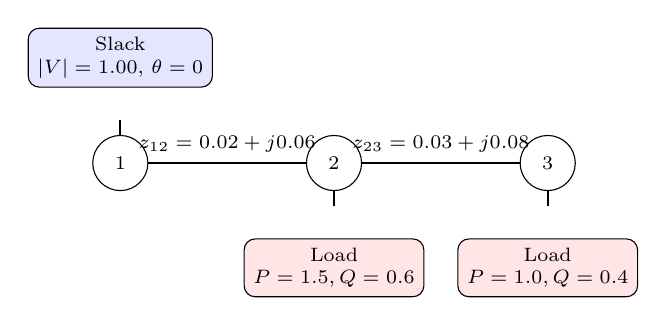
\begin{tikzpicture}[node distance=1.4cm and 2.0cm, every node/.style={font=\scriptsize}]
\tikzset{bus/.style={draw, circle, minimum size=0.7cm, fill=white}}
\tikzset{dev/.style={draw, rounded corners, align=center, minimum width=1.6cm, minimum height=0.7cm}}
\node[bus] (b1) {1};
\node[bus, right=of b1] (b2) {2};
\node[bus, right=of b2] (b3) {3};
\node[dev, above=0.6cm of b1, fill=blue!10] {Slack\\$|V|=1.00$, $\theta=0$};
\node[dev, below=0.6cm of b2, fill=red!10] {Load\\$P=1.5, Q=0.6$};
\node[dev, below=0.6cm of b3, fill=red!10] {Load\\$P=1.0, Q=0.4$};
\draw[thick] (b1) -- node[above]{$z_{12}=0.02+j0.06$} (b2);
\draw[thick] (b2) -- node[above]{$z_{23}=0.03+j0.08$} (b3);
\draw[thick] (b1) -- ++(0,0.55);
\draw[thick] (b2) -- ++(0,-0.55);
\draw[thick] (b3) -- ++(0,-0.55);
\end{tikzpicture}
\vspace{0.6em}
\begin{itemize}
  \item All quantities are in per-unit on a 100 MVA base.
  \item Bus 1: slack ($|V|=1$, $\theta=0$).
  \item Buses 2, 3: PQ buses.
  \item Goal: find $|V_2|, \theta_2, |V_3|, \theta_3$.
\end{itemize}
\end{frame}

% ============================================================
\begin{frame}{Three-bus example: build $Y_{\text{bus}}$}
Line admittances:
\begin{align*}
y_{12} &= 1/(0.02 + j0.06) = 5.00 - j15.00 \\
y_{23} &= 1/(0.03 + j0.08) = 4.10 - j10.93
\end{align*}
$Y_{\text{bus}}$ matrix:
\begin{equation*}
Y_{\text{bus}} = \begin{bmatrix}
\phantom{-}y_{12}            & -y_{12}        & 0 \\
-y_{12}        & \phantom{-}y_{12}+y_{23}  & -y_{23} \\
0              & -y_{23}        & \phantom{-}y_{23}
\end{bmatrix}
\end{equation*}
Each off-diagonal entry is $-y_{ij}$; each diagonal sums the admittances of branches touching that bus. The matrix is symmetric and (apart from the row/column corresponding to the slack) used directly in NR.
\end{frame}

% ============================================================
\begin{frame}{Three-bus example: NR sketch}
\begin{enumerate}
  \item \textbf{Initialize} (flat start): $|V_2| = |V_3| = 1$, $\theta_2 = \theta_3 = 0$.
  \item \textbf{Compute mismatch} $\Delta P_2, \Delta Q_2, \Delta P_3, \Delta Q_3$ from the PF equations.
  \item \textbf{Compute Jacobian} $J^{(0)}$ at the current $(|V|, \theta)$.
  \item \textbf{Solve} $J \, \Delta x = -F$ for $\Delta x = [\Delta\theta_2, \Delta\theta_3, \Delta|V_2|, \Delta|V_3|]$.
  \item \textbf{Update} $x \leftarrow x + \Delta x$.
  \item \textbf{Repeat} steps 2--5 until $\| F \|_\infty < 10^{-8}$.
\end{enumerate}
\vspace{0.5em}
\begin{block}{Numerical result (typical)}
$|V_2| \approx 0.965, \theta_2 \approx -3.0^\circ, |V_3| \approx 0.948, \theta_3 \approx -4.5^\circ$. Converges in 3 iterations.
\end{block}
\end{frame}

% ============================================================
\section*{6. pandapower preview}

\begin{frame}[fragile]{Minimal pandapower workflow}
\begin{lstlisting}
import pandapower as pp

net = pp.create_empty_network()
b1 = pp.create_bus(net, vn_kv=20.0, name="slack")
b2 = pp.create_bus(net, vn_kv=20.0, name="load1")
b3 = pp.create_bus(net, vn_kv=20.0, name="load2")

pp.create_ext_grid(net, bus=b1, vm_pu=1.0)
pp.create_line_from_parameters(
    net, b1, b2, length_km=1.0,
    r_ohm_per_km=0.08, x_ohm_per_km=0.24,
    c_nf_per_km=0.0, max_i_ka=0.4)
pp.create_line_from_parameters(
    net, b2, b3, length_km=1.0,
    r_ohm_per_km=0.12, x_ohm_per_km=0.32,
    c_nf_per_km=0.0, max_i_ka=0.4)

pp.create_load(net, bus=b2, p_mw=1.5, q_mvar=0.6)
pp.create_load(net, bus=b3, p_mw=1.0, q_mvar=0.4)

pp.runpp(net)
print(net.res_bus)
print(net.res_line)
\end{lstlisting}
\end{frame}

% ============================================================
\begin{frame}{Reading pandapower results}
\textbf{\code{net.res\_bus}} -- one row per bus:
\begin{itemize}
  \item \code{vm\_pu} -- voltage magnitude in per-unit
  \item \code{va\_degree} -- voltage angle in degrees
  \item \code{p\_mw}, \code{q\_mvar} -- net injection at the bus
\end{itemize}
\textbf{\code{net.res\_line}} -- one row per line:
\begin{itemize}
  \item \code{loading\_percent} -- $|I_{\max(\text{from},\text{to})}| / I_{\text{rated}} \times 100$
  \item \code{i\_from\_ka}, \code{i\_to\_ka}, \code{pl\_mw}, \code{ql\_mvar}
\end{itemize}
\vspace{0.5em}
\begin{alertblock}{Always do these three checks}
\begin{enumerate}
  \item \code{net.converged} is True.
  \item No \code{vm\_pu} outside $[0.95, 1.05]$ (unless expected).
  \item No \code{loading\_percent} above 100 (unless expected).
\end{enumerate}
\end{alertblock}
\end{frame}

% ============================================================
\section*{7. Limits and what's next}

\begin{frame}{What this lecture assumed}
\begin{enumerate}
  \item \warnitem \textbf{Balanced three-phase.} We treated each bus as a single complex voltage. This implicitly assumes the three phases are identical up to a $120^\circ$ rotation.
  \item \warnitem \textbf{Steady state.} No dynamics, no transient stability, no protection.
  \item \warnitem \textbf{Fixed topology.} No outages yet.
  \item \warnitem \textbf{AC, sinusoidal.} No DC links, no harmonics.
\end{enumerate}
\vspace{0.5em}
\begin{block}{When the balanced assumption is OK}
At transmission voltage levels with three-phase generation and roughly symmetric loads, the assumption is usually fine. We will see in L02--L04 that distribution networks (and especially LV microgrids) are a very different story.
\end{block}
\end{frame}

% ============================================================
\begin{frame}{Where we go from here}
\centering
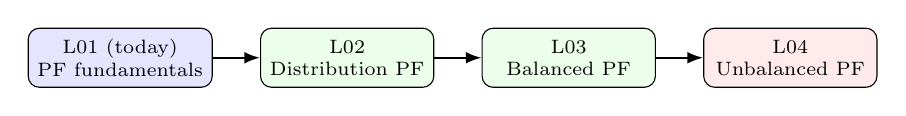
\begin{tikzpicture}[node distance=0.6cm and 0.6cm, every node/.style={font=\scriptsize}]
\tikzset{box/.style={draw, rounded corners, align=center, minimum width=2.2cm, minimum height=0.75cm}}
\tikzset{arrow/.style={-{Latex[length=2mm]}, thick}}
\node[box, fill=blue!10] (l1) {L01 (today)\\PF fundamentals};
\node[box, fill=green!8, right=of l1] (l2) {L02\\Distribution PF};
\node[box, fill=green!8, right=of l2] (l3) {L03\\Balanced PF};
\node[box, fill=red!8, right=of l3] (l4) {L04\\Unbalanced PF};
\draw[arrow] (l1) -- (l2);
\draw[arrow] (l2) -- (l3);
\draw[arrow] (l3) -- (l4);
\end{tikzpicture}
\vspace{1em}
\begin{itemize}
  \item \textbf{L02} -- radial feeders, R/X ratio, BFS, DER on distribution.
  \item \textbf{L03} -- when the balanced assumption is appropriate; positive sequence equivalents.
  \item \textbf{L04} -- symmetrical components, three-phase PF, VUF, why microgrids need it.
\end{itemize}
\end{frame}

% ============================================================
\begin{frame}{Homework}
\begin{block}{Required}
\begin{enumerate}
  \item By hand, write down $Y_{\text{bus}}$ for the three-bus system in this lecture.
  \item By hand, compute the power mismatch at the flat start.
  \item Reproduce the three-bus system in pandapower and run \code{pp.runpp(net)}. Confirm \code{net.converged} is True.
  \item Compare \code{net.res\_bus.vm\_pu} to the typical values quoted on the worked-example slide.
\end{enumerate}
\end{block}
\begin{block}{Optional}
\begin{enumerate}
  \item Double the line impedances and re-run. How does $|V|$ change at bus 3?
  \item Add a PV-type generator at bus 3 and observe how $\theta$ changes.
  \item Try \code{pp.runpp(net, algorithm="bfsw")} and compare voltages to NR. (We will come back to BFSW in L02.)
\end{enumerate}
\end{block}
\end{frame}

% ============================================================
\begin{frame}{Exit checklist}
\begin{enumerate}
  \item \checkitem I can explain what ``solving the power flow'' means in one sentence.
  \item \checkitem Given a one-line diagram, I can classify each bus as slack, PV, or PQ.
  \item \checkitem I can write down $Y_{\text{bus}}$ from line impedances.
  \item \checkitem I can state the power-flow equations and explain why they are nonlinear.
  \item \checkitem I know what Newton-Raphson does and what convergence means.
  \item \checkitem I can run \code{pp.runpp(net)} and read \code{net.res\_bus.vm\_pu} and \code{net.res\_line.loading\_percent}.
  \item \checkitem I understand that this lecture assumed three-phase balance and I know why L04 will revisit this.
\end{enumerate}
\end{frame}

% ============================================================
\begin{frame}{References}
\footnotesize
\begin{itemize}
  \item \textbf{Grainger \& Stevenson,} \emph{Power System Analysis}. The chapter on Newton-Raphson power flow.
  \item \textbf{Glover, Sarma, Overbye,} \emph{Power System Analysis and Design}. Bus admittance matrix and per-unit basics.
  \item \textbf{Wood, Wollenberg, Sheble,} \emph{Power Generation, Operation, and Control}. Decoupled and fast-decoupled PF.
  \item \textbf{pandapower documentation:} \url{https://pandapower.readthedocs.io} -- ``Balanced AC Power Flow''.
  \item \textbf{Tinney \& Hart, 1967.} \emph{Power Flow Solution by Newton's Method}, IEEE TPAS. The original NR-PF paper, still readable.
\end{itemize}
\end{frame}

\end{document}
